% ============================================================
%  SCHOLA DOMESTICA — Magister Mathematica
%  Level 1 | Week 12 | Day 3
%  Topic: Number Bonds to 6 — Addition and Subtraction Partners
% ============================================================
\documentclass[12pt, letterpaper]{article}

\usepackage[top=1in, bottom=1in, left=1in, right=1in]{geometry}
\usepackage[T1]{fontenc}
\usepackage[utf8]{inputenc}
\usepackage{lmodern}
\usepackage{microtype}
\usepackage{amsmath}
\usepackage{xcolor}
\usepackage{tikz}
\usepackage{array}
\usepackage{enumitem}
\usepackage{multicol}
\usepackage{mdframed}
\usepackage{fancyhdr}

\definecolor{scholared}{RGB}{160,30,30}
\definecolor{scholagold}{RGB}{180,140,40}
\definecolor{scholacream}{RGB}{253,248,235}
\definecolor{scholagreen}{RGB}{50,110,60}
\definecolor{scholablue}{RGB}{40,80,140}

\pagestyle{fancy}
\fancyhf{}
\renewcommand{\headrulewidth}{0.6pt}
\fancyhead[L]{\small\textcolor{scholared}{\textbf{Schola Domestica — Magister Mathematica}}}
\fancyhead[R]{\small\textcolor{scholared}{Level 1 · Week 12 · Day 3}}
\fancyfoot[C]{\small\textcolor{gray}{— \thepage\ —}}

\newcommand{\answerline}{\underline{\hspace{2.5cm}}}
\newcommand{\biganswerline}{\underline{\hspace{4cm}}}
\newcommand{\numbox}{\tikz{\draw[scholablue,thick](0,0)rectangle(1.2cm,0.85cm);}}

\newmdenv[
  backgroundcolor=scholacream,
  linecolor=scholared,
  linewidth=1.5pt,
  roundcorner=6pt,
  innertopmargin=8pt,
  innerbottommargin=8pt,
  innerleftmargin=10pt,
  innerrightmargin=10pt
]{lessonbox}

\newmdenv[
  backgroundcolor={rgb,255:red,235;green,245;blue,235},
  linecolor=scholagreen,
  linewidth=1.2pt,
  roundcorner=4pt,
  innertopmargin=6pt,
  innerbottommargin=6pt,
  innerleftmargin=8pt,
  innerrightmargin=8pt
]{enrichbox}

\begin{document}

\begin{center}
  {\LARGE\textbf{\textcolor{scholared}{Number Bonds to Six:}}}\\[4pt]
  {\Large\textcolor{scholagold}{\textit{The Family of Facts}}}\\[6pt]
  {\small Name: \biganswerline \hspace{1cm} Date: \answerline}
\end{center}

\vspace{4pt}
\noindent\textcolor{scholared}{\rule{\linewidth}{1pt}}
\vspace{4pt}

% IMAGE PROMPT (Beatrix Potter watercolour style):
% A mother rabbit sits between two smaller rabbits, all holding paws in a circle. Soft afternoon
% meadow light, wildflowers around them, white paper background, no text.

\begin{lessonbox}
\textbf{A number bond} shows how two parts make one whole.\\
\textbf{A fact family} shows all four number sentences from one bond.\\[6pt]
\noindent
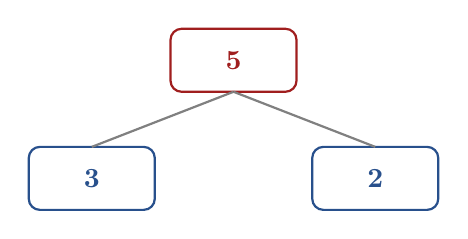
\begin{tikzpicture}
  \draw[scholared,thick,rounded corners=4pt](1.8,1.5)rectangle(3.4,2.3);
  \node[scholared] at (2.6,1.9) {\textbf{5}};
  \draw[scholablue,thick,rounded corners=4pt](0,0)rectangle(1.6,0.8);
  \node[scholablue] at (0.8,0.4) {\textbf{3}};
  \draw[scholablue,thick,rounded corners=4pt](3.6,0)rectangle(5.2,0.8);
  \node[scholablue] at (4.4,0.4) {\textbf{2}};
  \draw[gray,thick](0.8,0.8)--(2.6,1.5); \draw[gray,thick](4.4,0.8)--(2.6,1.5);
\end{tikzpicture}
\hspace{1cm}
\begin{tabular}{@{}l@{}}
$3 + 2 = 5$ \\
$2 + 3 = 5$ \\
$5 - 2 = 3$ \\
$5 - 3 = 2$
\end{tabular}
\end{lessonbox}

\bigskip

% ===== PART I: COMPLETE THE FACT FAMILIES =====
\noindent\textcolor{scholared}{\large\textbf{Part I — Fact Families}} \hfill \textit{(Problems 1–3, 4 sentences each)}

\medskip
\noindent\textit{Use the number bond to write all four number sentences.}

\bigskip

% Family 1: 1, 4, 5 — use this bond
\noindent\textbf{1.} Bond: \textbf{1}, \textbf{4}, whole = \textbf{5}

\medskip
\noindent\hspace{2em}
\begin{tabular}{@{}p{5.5cm} p{5.5cm}@{}}
$\numbox + \numbox = \numbox$ & $\numbox + \numbox = \numbox$ \\[10pt]
$\numbox - \numbox = \numbox$ & $\numbox - \numbox = \numbox$
\end{tabular}

\bigskip

% Family 2: 2, 4, 6
\noindent\textbf{2.} Bond: \textbf{2}, \textbf{4}, whole = \textbf{6}

\medskip
\noindent\hspace{2em}
\begin{tabular}{@{}p{5.5cm} p{5.5cm}@{}}
$\numbox + \numbox = \numbox$ & $\numbox + \numbox = \numbox$ \\[10pt]
$\numbox - \numbox = \numbox$ & $\numbox - \numbox = \numbox$
\end{tabular}

\bigskip

% Family 3: 3, 3, 6 (doubles — only 2 additions, 2 subtractions)
\noindent\textbf{3.} Bond: \textbf{3}, \textbf{3}, whole = \textbf{6}

\medskip
\noindent\hspace{2em}
\begin{tabular}{@{}p{5.5cm} p{5.5cm}@{}}
$\numbox + \numbox = \numbox$ & $\numbox - \numbox = \numbox$
\end{tabular}

\medskip\noindent\hspace{2em}\textit{(Why are there only 2 sentences this time? Because both parts are the same!)}

\bigskip\bigskip

% ===== PART II: MIXED SUBTRACTION FROM FAMILY KNOWLEDGE =====
\noindent\textcolor{scholared}{\large\textbf{Part II — Quick Subtraction Facts}} \hfill \textit{(Problems 4–11)}

\medskip
\noindent\textit{Use what you know about addition to help subtract.}

\bigskip

\noindent
\begin{tabular}{@{}p{3.3cm} p{3.3cm} p{3.3cm} p{3.3cm}@{}}
\textbf{4.}\; $5 - 1 =$ \numbox &
\textbf{5.}\; $5 - 4 =$ \numbox &
\textbf{6.}\; $6 - 2 =$ \numbox &
\textbf{7.}\; $6 - 4 =$ \numbox \\[12pt]
\textbf{8.}\; $6 - 3 =$ \numbox &
\textbf{9.}\; $4 - 0 =$ \numbox &
\textbf{10.}\; $5 - 2 =$ \numbox &
\textbf{11.}\; $6 - 6 =$ \numbox
\end{tabular}

\bigskip

% ===== PART III: WORD PROBLEMS =====
\noindent\textcolor{scholared}{\large\textbf{Part III — Story Problems}} \hfill \textit{(Problems 12–14)}

\medskip

\noindent\textbf{12.} There are \textbf{6} eggs in a basket. Mother uses \textbf{3} for baking. How many remain?

\medskip\noindent\hspace{2em} $6 - 3 =$ \numbox\ eggs

\bigskip

\noindent\textbf{13.} A branch had \textbf{5} cherries. A bird ate \textbf{2}. How many are left?

\medskip\noindent\hspace{2em} $5 -$ \numbox $=$ \numbox\ cherries

\bigskip

\noindent\textbf{14.} Write a subtraction story using the numbers 6 and 4:

\medskip\noindent\hspace{2em}\underline{\hspace{9cm}}

\medskip\noindent\hspace{2em} $6 - 4 =$ \numbox

\bigskip

\begin{enrichbox}
\textbf{\textcolor{scholagreen}{All fact families to 6 — say them aloud!}}\\[4pt]
$1{+}0=1, \; 1{-}0=1, \; 1{-}1=0$\\
$1{+}1=2, \; 2{-}1=1$\\
$1{+}2=3, \; 2{+}1=3, \; 3{-}1=2, \; 3{-}2=1$\\
$\ldots$ and so on through 6.\\[3pt]
\textit{Teacher: say the whole and one part; child says the missing part and the subtraction sentence.}
\end{enrichbox}

\vspace{0.3cm}
\noindent\textcolor{gray}{\small\textit{Ray's Primary Arithmetic — fact families and number bonds.}}

\end{document}
